\chapter{}
Jetzt etwas für Bastel intusiasten.
Wenn wir eine Metrik haben, dann können wir eine Topologie Basteln. 
Hirfür definieren wir die Menge:
$$Z : U_{x,l }:= x + l\mathbb{Z} = \{x + ln \mid n \in \mathbb{Z}\}, x \in \mathbb{Z}, l\in \mathbb{Z}, l \ge 1$$.

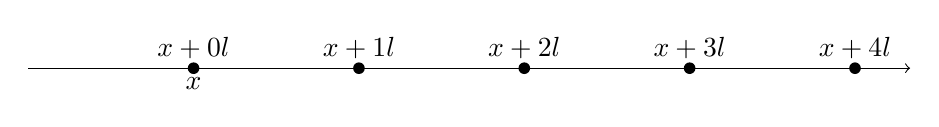
\begin{tikzpicture}[scale=0.7]
  % Parameter
  \def\x{2}   % Startwert
  \def\l{3}   % Schrittweite

  % Zahlengerade
  \draw[->] (-1,0) -- (15,0);

  % Punkte U_{x,l} = {x + l n}
  \foreach \n in {0,...,4}{
    \pgfmathsetmacro{\wert}{\x+\l*\n}
    \fill (\wert,0) circle (3pt)
      node[above] {$x+{\n}l$};
  }

  % Den Startwert extra beschriften
  \node[below] at (\x,0) {$x$};

\end{tikzpicture}

Das ganze ist sehr lustig, also unanschaulich. Also lustig für Mathematiker halt. 
Es kann natüich sein das einem der Witz an dem ganzen bis dato noch nicht aufgefallen ist. 
Aber nach dem man darauf aufmerksam gemacht wurde, ist es sehr lustig.
\bigskip

Betrachten wir also die Topologie:
$$\mathcal{T} := \{ O \subseteq \mathbb{Z} \mid \forall x \in O \exists l \in \mathbb{Z}, l \ge 1 : U_{x,l} \subseteq O\}$$
\begin{itemize}
    \item Sei $U_{k,l} \in \mathcal{T}, x \in U_{k,l}$. \\
    Dann gilt: $U_{x,l}=U_{k,l} : \text{ endlich}$
    Denn mit $n_x \in \mathbb{Z}: x = k + n_x l$. erhalten wir: \\
    \begin{itemize}
        \item Sei $y \in U_{x,l}: y = x + n_y l = U_{k,l} \ni k + (n_x + n_y)l$.
        \item Sei $y \in U_{k,l}: y = k + n_y l = U_{x,l} \ni x + (n'_y - n_{x})l$.
    \end{itemize}

    \item Das folgende ist eine Mengenspielerei und zur Erinnerung: Das gefällt uns!\\
    Wir betrachten also die Menge $$\mathbb{Z} \setminus U_{k,l} \in \mathcal{T}: \mathbb{Z} \setminus U_{k,l} 
    = \underset{x= k+1}{\overset{k+l-1}{\bigcup}} U_{x,l} \in \mathcal{T}$$
    Und weiters 
    $$\mathbb{Z}\setminus\{1,-1\} = \underset{p \in \mathbb{P}}{\bigcup} U_{0,p} \dots \{1,-1\}$$
    Hir ist wichtig zu bemerken das die Geometrische Progession unendlich ist und die Menge $\{-1,1\}$ nicht. 
    Das bedute $\{1,-1\} \notin \mathcal{T}$.\\
    $= \underset{p \in \mathbb{P}}{\bigcup}\underset{\in \mathcal{T}}{\mathbb{Z}\setminus{U_{0,p}}}$. 
    $\mathbb{P}:= \{p \in \mathbb{N} \mid p \text{ Prim} \,\} \Rightarrow \mathbb{P} \text{ unendlich}$.
    Damit haben wir auch gezeigt das die Menge der Primzahlen unendlich ist.
    
\end{itemize}

\dfn{Halbordnung auf der Menge der Topologien}{

Sei $X$ eine Menge. 
Betrachte 
$\mathbb{T}(x) := \{\mathcal{T}(X)\subset \mathcal{P}(X)\mid \mathcal{T} \text{Topologie auf } X\}$.  
Dan nennen wir 
\begin{enumerate}
  \item $\mathbb{T}(X)$ ist eine halbgeordnet mit $\subseteq$ 
  Seien $\mathcal{T}_1, \mathcal{T}_2 \in \mathbb{T}(x)$
  Dann ist $\mathcal{T}_1 \subseteq \mathcal{T}_2$ eine Hablbordnung mit: 
  $\forall O \subseteq X: O \in \mathcal{T}_1 \Rightarrow \mathcal{T}_2$
  \item Weiters betrachten wir
  $\{\emptyset, X\} \in \mathbb{T} \text{ und } \forall \mathcal{T} \in \mathbb{T}: \{\emptyset,X\}\subset \mathcal{T}$
  $\mathcal{P}(X) \in \mathbb{T}(X) $ und $\forall \mathcal{T} \in \mathbb{T}(X): \mathcal{T}\subset \mathbb{P}$
  \item $\mathbb{V} \subseteq \mathbb{T}(X)$ Dann gilt: $\mathbb{V} \neq \emptyset\footnote{\text{ um Sonderfälle zu vermeiden}}$ 
  hat ein Infimum in $\mathbb{T}(X)$.
\end{enumerate}
\begin{proof}
  Den letzten Teil der Definition wollen wir jetzt beweisen. 
  - Eine Definition die man erst beweisen muss, ist schon lustig.- \\
  \begin{enumerate}
    \item Im ertsen schritt wählen wir einen Kanditaten  $\mathbb{V}$ in $\mathbb{T}(X)$ 
    Hierfür betrachten wir $\bigcap \mathbb{V} \in \mathbb{T}(X)$
    \begin{itemize}
      \item[(i)] Sei $V \in \mathbb{V}$ Dann ist $\emptyset \in V$ und $X \in V \Rightarrow \emptyset \in \bigcap \mathbb{V}$.
      und auch $x \in \bigcap \mathbb{V}$ 
      \item[(ii)] $\mathcal{V} \subseteq \bigcap \mathbb{V}$ 
      Sei $V \in \mathbb{V}$. Dann gilt:
    $$ \mathcal{V} \subseteq V \Rightarrow \bigcup \mathcal{V} \in V \Rightarrow \bigcup \mathcal{V} \in \bigcap \mathbb{V}.$$

      \item[(iii)]
    $\mathcal{V} \subseteq \bigcap \mathbb{V}$ endlich.  
    Sei $V \in \mathbb{V}$. Dann gilt:
    $$ \mathcal{V} \subseteq V \Rightarrow \bigcap \mathcal{V} \in V \Rightarrow \bigcap \mathcal{V} \in \bigcap \mathbb{V}.$$
    \end{itemize}
    Damit sehen wir das unser gewählter Kandidat in der Grundmenge ist - was ihn zu einem guten Kanditatenmacht -.
    \item Wir zeigen jetzt das $\bigcap \mathbb{V}$ eine Untere Schranke ist.
   Sei $\mathcal{V}  \in \mathbb{V} :$ Dann $\bigcap \mathbb{V} \in \mathbb{T}(X)$ \\
   Sei $\mathcal{V}  \in \mathbb{V} :$ Es fehlt zu zeigen das $\mathcal{V} \subseteq \bigcap \mathbb{V}$.
   Sei $V \in \bigcap \mathbb{V} :$ Dann $V \in \mathcal{V}$
    \item Wir zeigen jetzt noch das $\bigcap \mathbb{V}$ nicht nur ihrgend eine unter schranke ist
    sondern die größte.
    Sei $\mathcal{W} \in \mathbb{T}(X)$ eine untere Schranke von $\mathbb{V}$ - hir ihrgend eine unter schranke -.
    Was bedeutet es eine untere Schranke zu sein?
    $$\forall V \in \mathbb{V}: \mathcal{W} \subseteq V$$
    Zu zeigen ist jetzt: $\mathcal{W} \subseteq \bigcap \mathbb{V}$.
    Das heißt $\forall \mathcal{V} \in \mathbb{V}: \mathcal{W} \subseteq \mathcal{V}$.
    Das heißt wiederum $\forall \mathcal{V} \in \mathbb{V}, \forall O \in \mathcal{W}: O \in \mathcal{V}$.
    also $\forall O \in \mathcal{W}: O \in \bigcap \mathbb{V}$.
    Das heißt $\mathcal{W} \subseteq \bigcap \mathbb{V}$.
  \end{enumerate}
\end{proof}
}

\nt{ Jede Menge, die ein Infimum hat und ein größtes Element, dann hat jede Teilmenge auch ein Supremum.}

An der Bemerkung angelehnt, wollen wir jetzt noch zeigen, dass jede Teilmenge von $\mathbb{T}(X)$ auch ein Supremum hat.

\begin{corollary}{ }
  JJede Teilmenge von $\mathbb{T}(X)$ hat ein Supremum.
\end{corollary}